\chapter{SAR Polarimetry}\label{chp:obs}%\Cref{sec:pr_obs}
%The main observational data used within this thesis are of four different kinds: precipitation, discharge, 

%------------------------------------
%	PRECIPITATION OBS
%------------------------------------

\section{Electromagnetic radiation}
\section{SAR system characteristics} \label{sec:pr_obs}
%\subsection*{Phase and Polarization}
%Precipitation is probably the most difficult of all atmospheric climate variables to measure reliably, due to the huge spatio-temporal variability (especially in summer) and to the physical difficulty of setting up and maintaining a dense network of high-maintenance sensors. In our multi-model approach
\section{Polarimetry}

%\subsection*{Generating Polarimetric Parameters in SNAP}
	\begin{figure}[H]
    \centering
    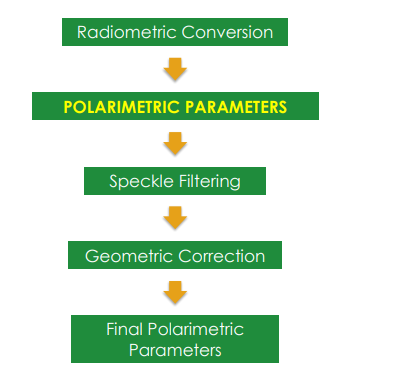
\includegraphics[width=0.4\textwidth]{figures/images/snap.PNG}
    \decoRule
    \caption[Generating Polarimetric Parameters in SNAP]{Generating Polarimetric Parameters in SNAP.}
    \label{fig:undercatch}
\end{figure}

	
	%\begin{wrapfigure}{l}{0.25\textwidth}
%\includegraphics[width=0.9\linewidth]{figures/PolSAR.jpg}
%\caption{Ttulo 1}
%\label{F:figuranotexto}
%\end{wrapfigure}


\subsection*{Example math equations}
%-----------------------------------------------------------
%\begin{align*}
%L(\alpha,  \lambda|  \bm{x})&=\prod_{i=1}^n{f(x_i|\alpha, \lambda )}\\
                                 %&= \prod_{i=1}^n\left[\frac{\lambda^{\alpha}}{\Gamma(\alpha)}\,x_i^{\alpha-1}\exp\left\{-\lambda x_i\right\}\right]\\
%&=\left(\frac{\lambda^{\alpha}}{\Gamma(\alpha)}\right)^n\prod_{i=1}^nx_i^{\alpha-1}\times \exp\left\{-\left(\lambda\sum_{i=1}^n x_i \right)\right\}
%\end{align*}
%%----------------------------------------------------------
\begin{align}
\label{eq:em}
\ell(\alpha, \lambda| \bm{x}) &=\log\left[\left(\frac{\lambda^{\alpha}}{\Gamma(\alpha)}\right)^n\prod_{i=1}^nx_i^{\alpha-1}\times \exp\left\{-\left(\lambda\sum_{i=1}^n x_i \right)\right\}\right]\nonumber\\
&=\log\left(\frac{\lambda^{\alpha}}{\Gamma(\alpha)}\right)^n+\log\left[\prod_{i=1}^nx_i^{\alpha-1}\right]-\lambda\sum_{i=1}^nx_i\nonumber\\
&=n\log\left(\frac{\lambda^{\alpha}}{\Gamma(\alpha)}\right)+(\alpha-1)\log\prod_{i=1}^nx_i-\lambda\sum_{i=1}^nx_i\nonumber\\
&=n\log(\lambda^{\alpha})-n\log(\Gamma(\alpha))+(\alpha-1)\sum_{i=1}^n\log(x_i)-\lambda\sum_{i=1}^nx_i\nonumber\\
&=n\alpha\log \lambda -n\log(\Gamma(\alpha)) +(\alpha-1)\sum_{i=1}^n\log(x_i)-\lambda\sum_{i=1}^nx_i.
	\end{align}
%----------------------------------------------------------
\begin{figure}
    \centering
    \includegraphics[width=0.5\textwidth]{figures/images/PolSAR.jpg}
    \decoRule
    \caption[Example plot]{Example plot.}
    \label{fig:undercatch}
\end{figure}

%-------------------------------------------------------

%\begin{table}[h]
%\centering
%\caption{\label{tab1}Comparação de tempos. }
%\begin{tabular}{l c c }
%\toprule[1pt] \textbf{Amostra (N)} \ \ \  \ \ \  & \textbf{Tempo de Execução (C)}\ \ \ \ \ \ \  &\textbf{Tempo de Execução (Ox)} \\\midrule[0.5pt]
%$20$ & 7.6810 s  &  5.01 s \\
%$30$ & 9.6260 s     & 5.34 s \\
%$50$ &  10.0310 s & 5.99 s \\
%$100$ & 15.5420 s & 8.07 s \\
%$200$ & 20.5860 s & 9.64 s \\
%$500$ & 29.0890  s & 15.12 s \\
%\bottomrule[1pt]
%\end{tabular}
%\caption[Precipitation datasets]{List of datasets used in the analysis of daily precipitation uncertainty carried over i}\label{tab:1}
%\end{table}
%------------------------------------------------------


%\begin{table}[]
%\centering
%\begin{tabular}{@{}llll@{}}
%\toprule
%Dataset name & Period & Spatial res. & Data source \\ \midrule
%E-OBS        & 2000--2016 & \ang{0.25}                            & Station data \\
%EURO4M-APGD  & 2000--2008 & \SI{5}{\kilo\metre}                   & Station data \\
%HMR          & 2000--2013 & \SI{5.5}{\kilo\metre}                 & Reanalysis \\
%ARCIS        & 2000--2015 & \textasciitilde{} \SI{5}{\kilo\metre} & Station data \\
%CHIRPS       & 2000--2016 & \ang{0.05}                            & Station data + satellite \\
%CPC          & 2000--2016 & \ang{0.5}                             & Station data \\
%CMORPH       & 2000--2016 & \ang{0.25}                            & Satellite \\
%PERSIANN-CDR & 2000--2016 & \ang{0.25}                            & Satellite \\ \bottomrule
%\end{tabular}
%\caption[ Italy]{List of datasets used in the analysis of daily precipitation uncertainty  references.}\label{tab:2}
%\end{table}




